%TODO: ARREGLAR EJERCICIO 1B
\documentclass{article}
\usepackage[utf8]{inputenc}
\usepackage[spanish]{babel}
\usepackage{graphicx, graphics, float, hyperref}
\usepackage{listings}
\usepackage[a4paper, total={6in, 10in}]{geometry}

\title{SSO Práctica 1 Sesión 2}
\author{Andrés Merlo Trujillo}
\date{}
\hypersetup{
    colorlinks=true,
    linkcolor=black,
}

\begin{document}

\maketitle

\tableofcontents

\newpage
%\addcontentsline{toc}{section}{Ejercicio 1}
%\section*{Ejercicio 1}
%\begin{figure}[H]
%    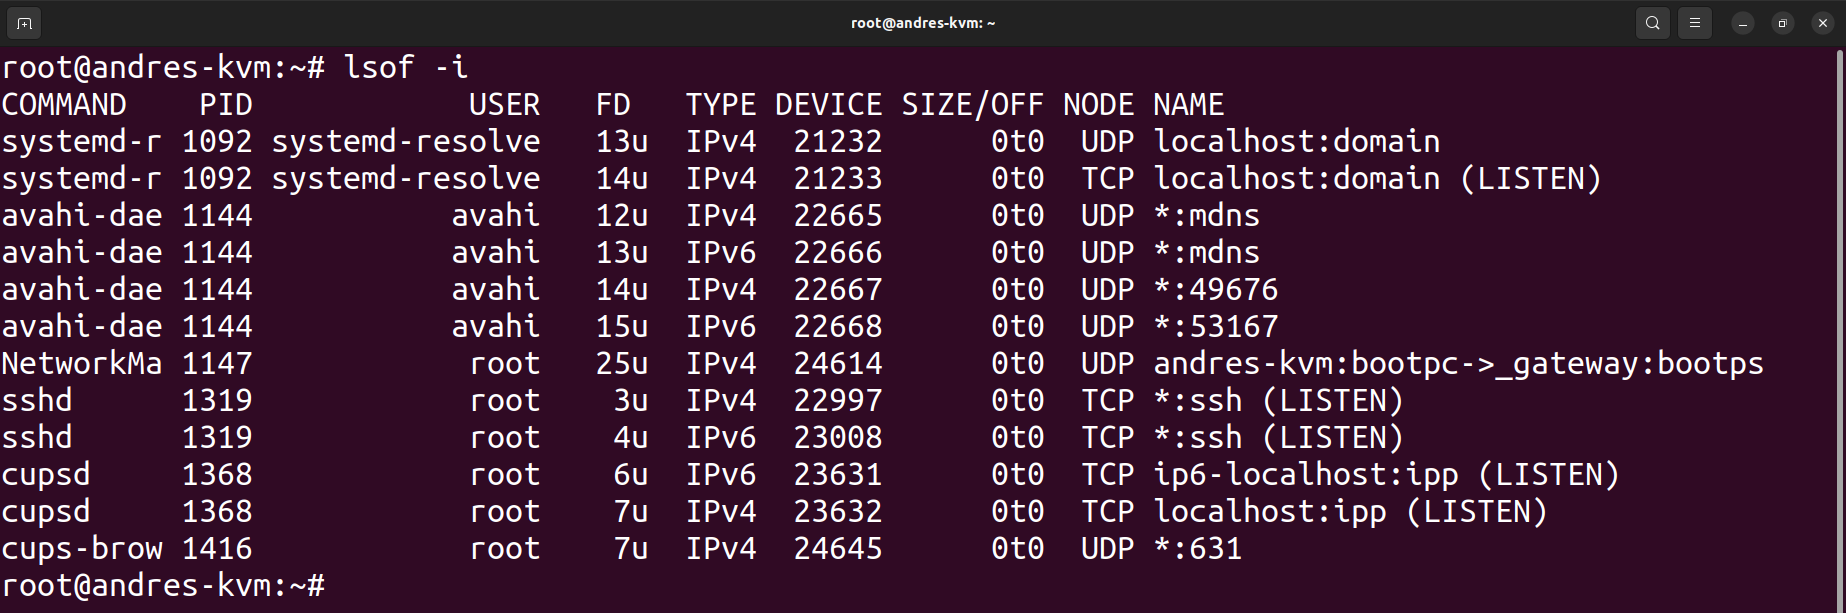
\includegraphics[width=\textwidth]{imagenes/lsofi.png}
%\end{figure}

\addcontentsline{toc}{section}{Ejercicio 1}
\section*{Ejercicio 1}


\end{document}

%\begin{figure}[H]
%    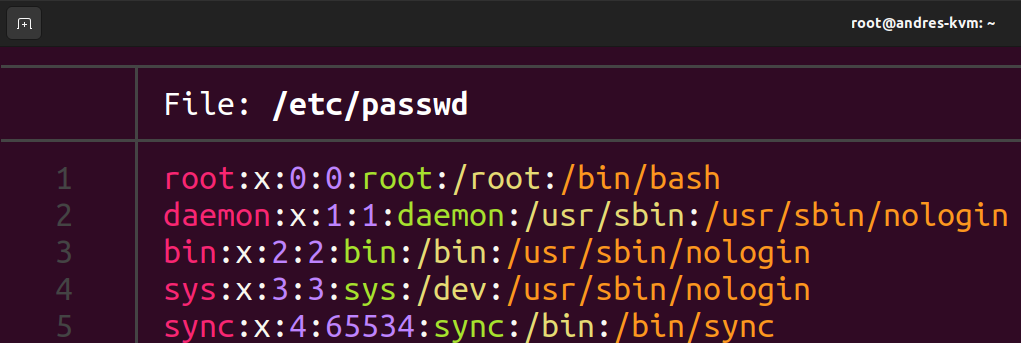
\includegraphics[width=\textwidth]{imagenes/passwdfile.png}
%    \caption{Ejemplo de entradas en el archivo.}
%\end{figure}